\chapter{리눅스 커널}
\section{리눅스 아키텍처}
\begin{itemize}
    \item \textbf{하드웨어 계층}\newline
        CPU와 메인 메모리, 디스크, NIC, I/O 디바이스 모두를 총칭한다.
    \item \textbf{커널 계층}\newline
        하드웨어 계층과 사용자 영역 계층의 사이에 위치한다.\newline
        이번 chapter에서 다루는 계층이다.
    \item \textbf{사용자 영역 계층}\newline
        shell 및 ps, ssh 같은 유틸리티, GUI를 비롯해 
        대부분의 앱이 실행되는 계층이다.
\end{itemize}

\begin{flushleft}
    다른 계층간 인터페이스는 리눅스 운영체제 패키지의 일부이다.
    그 중 커널과 사용자 영역 계층 인터페이스를 \textbf{시스템 콜}(system call)이라 부른다.
\end{flushleft}

\begin{flushleft}
    하드웨어와 커널 사이의 인터페이스는 시스템 콜과 달리 
    단일 인터페이스가 아니라 
    일반적으로 하드웨어별 그룹화된 개별 인터페이스 모음으로 구성된다.

    \begin{itemize}
        \item CPU 인터페이스
        \item main memory 인터페이스
        \item 네트워크 인터페이스와 드라이버
        \item 파일시스템과 블록 디바이스 드라이버 인터페이스
        \item 캐릭터 디바이스, 하드웨어 인터럽트, 
        키보드, 터미널, 기타 I/O 등의 입력 디바이스를 위한 디바이스 드라이버
    \end{itemize}
\end{flushleft}
\newpage

\begin{figure}
    \centering
    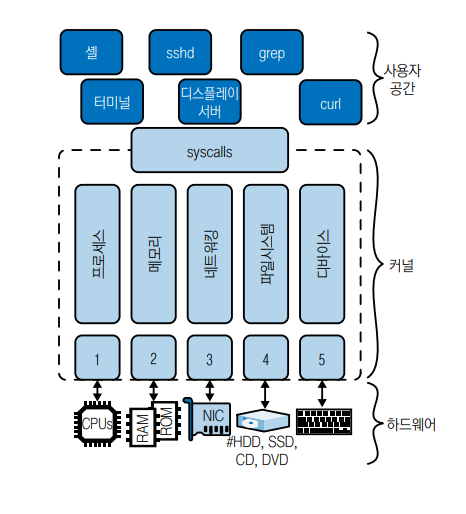
\includegraphics[width=10cm]{resource/2-1.png}
    \caption{리눅스 아키텍처 개요}
\end{figure}
\begin{flushleft}
    일반적으로 \textbf{커널 모드}는 추상화를 제한함으로써 빠르게 실행함을 의미하는 반면, 
    \textbf{사용자 모드}는 상대적으로 느리지만 더 안전하고 편리한 추상화를 의미한다.
    대부분의 경우 커널 모드를 신경쓰지 않아도 사용에 지장은 없지만,
    커널과 상호 작용하는 방법(시스템 콜)을 아는 것은 중요하다.
\end{flushleft}


\section{CPU 아키텍처}
\subsection{x86-64 아키텍처}
\begin{flushleft}
    x86과 amd64를 합쳐서 x86-64라고 부른다.
    x86은 인텔 32-bit ISA이며, amd64는 64-bit ISA이다.
    대부분의 경우 사용되는 CPU이며 오래전부터 사용되어왔고, 
    CISC(Complex Instruction Set Computer) 아키텍처 에너지 효율은 높지 않다.
\end{flushleft}

\subsection{ARM 아키텍처}
\begin{flushleft}
    RISC(Reduced Instruction Set Computer) 아키텍처이며 적은 명령어 집합을 사용한다.
    RISC는 CISC에 비해 전력 소모가 적다는 장점을 가지고 있으며, 
    저전력 환경(임베디드, 휴대용 디바이스)에서 널리 사용된다.
\end{flushleft}


\subsection{RISC-V 아키텍처}
\begin{flushleft}
    ARM과 달리 개방형 RISC 표준으로 아직 널리 사용되지는 않는다. 
    다만 ARM과 달리 라이센스 비용이 없어 주목받고 있다.
\end{flushleft}


\section{커널 구성요소}
커널 코드에서 제공하는 주요 기능은 다음과 같다.

\begin{itemize}
    \item \textbf{프로세스 관리}: 실행 파일을 기반으로 프로세스 시작
    \item \textbf{메모리 관리}: 프로세스에 메모리 할당 및 파일을 메모리에 매핑
    \item \textbf{네트워킹}: 네트워크 인터페이스 관리 및 네트워크 스택 제공
    \item \textbf{파일시스템}: 파일 관리를 제공하고, 파일 생성과 삭제 지원
    \item 케릭터 디바이스와 디바이스 드라이버 관리
\end{itemize}

\subsection{프로세스 관리}
\begin{flushleft}
    커널에는 프로세스 관리와 관련된 부분이 여러개 있다. 
    그중 일부는 인터럽트 같은 CPU 아키테기처 관련 사항을 처리하고, 
    다른 부분은 프로그램 실행과 스케줄링에 중점을 둔다.
\end{flushleft}

\begin{flushleft}
    일반적으로 프로세스는 실행 가능한 프로그램(또는 바이너리)을 기반으로 하며,
    사용자가 대면하는 유닛(unit)이다. 
    반면에 스레드는 프로세스 컨텍스트상 실행 유닛을 말한다. 
    멀티스레드라는 용어가 존재하는 것 처럼 
    프로세스에는 여러 실행 유닛이 병렬로 실행되며 
    이는 잠재적으로 다른 CPU에서 실행될 수 있다.
\end{flushleft}

\begin{flushleft}
    아래는 실제 리눅스에서 프로세스를 관리하는 단위이다.
\end{flushleft}

\begin{itemize}
    \item \textbf{세션}\newline
        하나 이상의 프로세스 그룹을 포함하고 선택적으로 tty가 연결된 
        상위 수순의 사용자 대면 유닛.
        커널은 textbf{세션 ID}(SID)라는 번호를 통해 세션을 식별한다.
    \item \textbf{프로세스 그룹}\newline
        하나 이상의 프로세스가 포함되어 있으며, 
        한 세션에는 foreground 프로세스 그룹이 둘 이상일 수 없다.
        커널은 \textbf{프로세스 그룹 ID}(PGID)라는 숫자를 통해 프로세스 그룹을 식별한다.
    \item \textbf{프로세스}\newline
        여러 리소스(주소 공간, 하나 이상의 스레드, 소켓 등)를 그룹으로 추상화한 것이며, 
        커널은 /proc/self를 통해 현재 프로세스를 사용자에게 노출한다.
        커널은 \textbf{프로세스 ID}(PID)라는 숫자를 통해 프로세스를 식별한다.
    \item \textbf{스레드}\newline
        커널에 의해 프로세스로 구현된 유닛을 말한다.
        즉 스레드를 나타내는 전용 데이터 구조는 없다.
        오히려 스레드는 특정 리소스(ex - 메모리, signal handler)를 다른 프로세스와 공유하는 프로세스다.
        커널은 \textbf{스레드 ID}(TID)와 \textbf{스레드 그룹}(TGIO)를 통해 스레드를 식별하며,
        공유된 TGID 값은 멀티스레드 프로세스를 의미한다.
    \item \textbf{태스크}\newline
        커널에는 sched.h에 정의된 \textbf{task\_struct}라는 데이터 구조가 있으며, 
        이는 프로세스와 스레드 구현의 기반을 형성한다.
        이 데이터 구조는 스케줄링 관련 정보, 식별자(ex - PID, TGID), signal handler,
        성능이나 보안과 관련된 기타 정보를 수집한다.
        즉, 앞서 언급한 모든 유닛은 태스크에서 파생되거나 고정(anchor)된다.
        하지만 캐스크는 커널 외부에 그대로 노출되는 일이 없다.
\end{itemize}

\begin{flushleft}
    실제로 그러한지 실습해보자.\newline
    아래는 ps -j로 확인할 수 있는 정보이다.
\end{flushleft}

\begin{figure}[h]
    \centering
    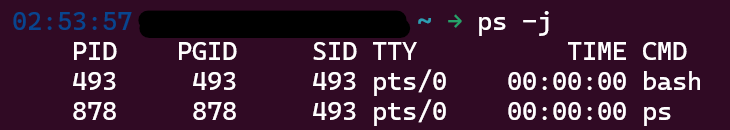
\includegraphics[width=10cm]{resource/ps-example.png}
    \caption{실습}
    \begin{enumerate}
        \item bash 셸 프로세스의 PID, PGID, SID는 모두 -이다.\newline
            ls -la /proc/493/task/493/로 태스트 수준의 정보를 수집할 수 있다.
        \item ps 프로세스의 PID/PGID는 878이고 SID는 셀과 동일하다.
    \end{enumerate}
\end{figure}

\begin{flushleft}
    리눅스의 작업 데이터 구조가 스케줄링과 관련된 정보를 준비된 상태로 가지고 있음을 
    앞에서 언급했던 적이 있다.
    이는 항상 프로세스는 아래 그림처럼 
    특정한 상태(state)에 있음을 의미한다.
\end{flushleft}
\newpage

\begin{figure}[h]
    \centering
    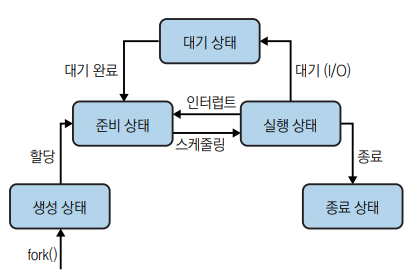
\includegraphics[width=10cm]{resource/2-2.png}
    \caption{리눅스 프로세스 상태}
\end{figure}

\begin{flushleft}
    이벤트가 일어날 때마다 상태 전환이 일어난다.
    예를 들어 실행 중인 프로세스가 일부 I/O 작업을 진행했으나 
    이를 실행할 수 없을 때 대기 상태로 전환될 수 있다.
\end{flushleft}

\begin{flushleft}
    보다 상세한 리눅스 프로세스의 상태는 
    다음 글 \href{https://www.baeldung.com/linux/process-states}{리눅스 프로세스 상태}를 참고하라
\end{flushleft}


\subsection{메모리 관리}
\begin{flushleft}
    가상 메모리는 시스템이 물리적으로  가지고 있는 것 보다
    더 많은 메모리를 갖고 있는 것처럼 보이게 한다.
    사실 모든 프로세스는 가성 메모리를 얻는다.
    물리 메모리와 가상 메모리는 모두 \textbf{페이지}(page)라고 부르는 고정길이 묶음으로 나뉜다.
\end{flushleft}

\begin{figure}[h]
    \centering
    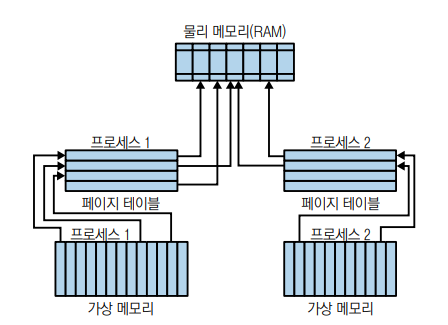
\includegraphics[width=10cm]{resource/2-3.png}
    \caption{가상 메모리 관리 개요}
\end{figure}
\newpage

\begin{flushleft}
    이전 페이지의 그림은 고유한 페이지 테이블이 있는 두 프로세스의 가상 주소 공간을 보여준다.
    이 페이지 테이블은 프로세스의 가상 페이지를 주 메모리의 물리적 페이지에 매핑(mapping)한다.
\end{flushleft}

\begin{flushleft}
    각 프로세스 수중의 페이지 테이블을 통해 여러 가상 페이지가 동일한 물리적 페이지를 가리킬 수 있다.
    즉, 기존 공간을 최적으로 사용하면서 
    각 프로세스에 그들의 페이지가 실제로 RAM에 존재한다는 환상을 효과적으로 일으키는 방법으로
    이는 실제 가지고 있는 물리 메모리 용량 이상으로 메모리를 사용할 수 있게 하여 
    어떤 의미로는 메모리 관리의 핵심이라 할 수 있다.
\end{flushleft}

\begin{flushleft}
    CPU가 프로세스의 가상 페이지에 접근할 때마다
    원칙적으로 CPU는 프로세스가 사용하는 가상 주소를 이에 해당하는 실제 주소로 변환해야 한다.
    이 절차의 속도를 높히기 위해 요즘 CPU 아키텍처는 TLB(translation lookaside buffer)라는
    조회용 on-chip을 지원한다.
    TLB는 작은 cache로 mapping된 주소가 누락된 경우 CPU가 프로세스 페이지 테이블을 통해
    페이지의 실제 주소를 계산하고 TLB를 업데이트한다.
\end{flushleft}

\begin{flushleft}
    전통적으로 리눅스의 기본 페이지 크기는 4KB였으나 커널 버전 2.6.3 부터는 그 이상의 대형 페이지를 지원한다.
    예를 들어 64-bit 리눅스에서는 프로세스당 총 128TB의 가상 주소 공간을 사용할 수 있으며,
    약 64TB의 물리 메모리를 사용할 수 있다.
\end{flushleft}

\begin{flushleft}
    아래는 /proc/meminfo 인터페이스를 사용해 메모리 관련 정보를 파악하는 예시이다.
\end{flushleft}

\begin{figure}[h]
    \centering
    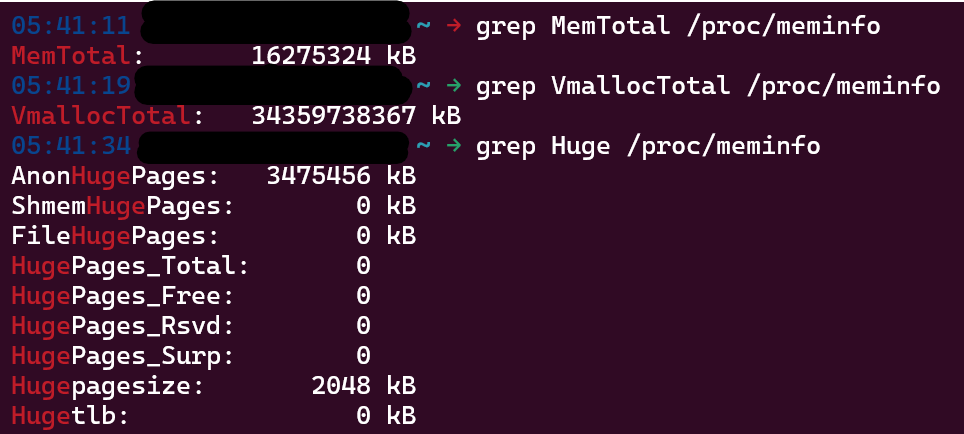
\includegraphics[width=10cm]{resource/mem-example.png}
    \caption{/proc/meminfo 실습}
\end{figure}

\begin{enumerate}
    \item 물리적 메모리에 대한 세부 정보 나열한다. 약 16GB이다.
    \item 가상 메모리에 대한 세부 정보를 나열한다. 약 34TB이다.
    \item 대형 페이지 정보를 나열한다. 여기서 페이지 크기는 2MB이다.
\end{enumerate}
\newpage

\subsection{네트워킹}
리눅스의 네트워크 스택은 계층화된 아키텍처를 따른다.

\begin{itemize}
    \item \textbf{소켓}\newline
        추상화 커뮤니케이션을 위해 필요
    \item \textbf{TCP(Transmission Control Protocol) 및 UDP(User Datagram Protocol)}\newline
        각각 연결형 통신과 비연결형 통신
    \item \textbf{인터넷 프로토콜}(IP)\newline
        기기의 주소 지정을 위해 필요
\end{itemize}

\begin{flushleft}
    이와 같은 세 가지 작업은 커널이 처리하는 모든 것이다.
    HTTP나 SSH 같은 애플리케이션 계층 프로토콜은 주로 사용자 영역에서 구현된다.
\end{flushleft}

\subsection{파일시스템}
\begin{flushleft}
    리눅스는 파일시스템을 사용해 HDD, SDD, 플래시 메모리 같은 
    저장 디바이스의 파일과 디렉터리를 구성한다. 
    ext4, btrfs, NTFS 같은 다양한 융형의 파일시스템이 있으며 
    동일한 파일 시스템의 인스턴스도 여러 개 사용할 수 있다.
\end{flushleft}
\begin{flushleft}
    가상 파일시스템(Virtual File System, VFS)은 원래 여러 파일시스템 유형과 인스턴스를 지원하기 위해 도입되었다.
    VFS의 최상위 계층은 열기, 닫기, 읽기, 쓰기 기능 등 공통 API 추상화를 제공하며, 
    VFS의 최하위 계층은 주어진 파일시스템에 대한 \textbf{플러그인}이라고 불리는 파일시스템 추상화다.
\end{flushleft}

\subsection{디바이스 드라이버}
\begin{flushleft}
    \textbf{드라이버}는 커널에서 실행되는 코드이다.
    그 역할을 키보드, 마우스, HDD 같은 실제 하드웨어 디바이스나
    /dev/pts/ 아래의 의사 터미널 같은 의사 디바이스(pseudo-device)를 관리하는 것이다.
    의사 디바이스는 가상의 디바이스지만 실제 디바이스처럼 취급될 수 있다.
\end{flushleft}

\begin{flushleft}
    드라이버는 커널에 정적으로 빌드될 수도 있고,
    필요할 때 동적으로 로드될 수 있도록 커널 모듈로 빌드될 수 있다.
\end{flushleft}
\newpage


\subsection{시스템 콜}
\begin{flushleft}
    터미널에 \textbf{touch test.txt}를 입력하거나
    앱 중 하나가 원격 시스템에서 파일 컨텐츠를 다운로드하길 원한다면
    결국에는 '파일 생성'이나 '어떤 주소에서 모든 바이트 읽기'와 같은 상위 수준의 명령을
    일련의 구체적인 아키텍처 종속 단계로 전환하도록 리눅스에 요청하게 된다.
    즉, \textbf{커널이 노출하는 서비스 인터페이스와 해당 사용자 영역의 엔티티 호출}은
    시스템 호출의 모음이라 하며, \textbf{시스템 콜}이라 부른다.
\end{flushleft}

\begin{flushleft}
    리눅스에 수백개의 시스템 콜이 존재하며,
    일반적으로 이러한 시스템 콜을 직접 호출하는 대신 \textbf{C 표준 라이브러리}라는 것을 통해 호출한다.
    표준 라이브러리는 wrapper 기능을 제공하며 glibc나 musl 같은 다양한 구현체에서 사용할 수 있다.
\end{flushleft}

\begin{flushleft}
    \textbf{wrapper 라이브러리는 시스템 콜 실행의 반복적인 저수준 처리를 다룬다는 중요한 작업을 수행}한다.
    시스템 콜은 소프트웨어 인터럽트로 구현되기 때문에 예외 처리기로 제어권을 넘기는 예외를 발생시킨다.
    시스템 콜이 호출될 때마다 처리해야할 여러 단계가 존재하며 아래의 예시를 보면서 짚어보자.
\end{flushleft}

\begin{figure}[h]
    \centering
    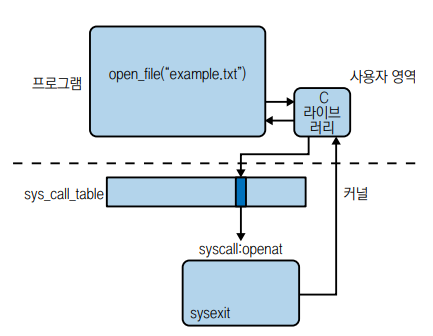
\includegraphics[width=10cm]{resource/2-4.png}
    \caption{리눅스의 시스템 콜 실행 단계}
\end{figure}

\begin{enumerate}
    \item syscall.h와 아키텍처 종속 파일(커널은 시스템 콜 테이블이라 부르는 파일 사용)에 정의되어
        메모리에 있는 함수 포인터 배열(sys\_call\_table이라는 변수에 저장됨)을 통해
        시스템 콜과 해당 처리기를 추적한다. 
    \item 시스템 콜 멀티플랙서처럼 동작하는 system\_call() 함수를 실행하면
        먼저 하드웨어 컨텍스트를 스택에 저장한 다음 검사를 수행하고(ex - 추적이 되는지 여부),
        그 이후에 sys\_call\_table의 각 시스템 콜 번호의 index가 가리키는 함수로 점프한다
    \item sysexit로 시스템 콜이 완료되면 wrapper 라이브러리는 하드웨어 컨텍스트를 복원하고,
        프로그램 실행은 사용자 영역에서 다시 사작된다.
\end{enumerate}

\begin{flushleft}
    위와 같은 단계에서 주목해야할 것은
    시간이 많이 소요되는 작업인 커널 모드와 사용자 영역 모드간의 전환이다.
\end{flushleft}

\begin{flushleft}
    시스템 콜이 실제로 어떻게 사용되는지 보는 구체적 예시를 보자.
    \textbf{strace}를 사용해 내부 동작을 확인해보자.
\end{flushleft}

\begin{figure}[h]
    \centering
    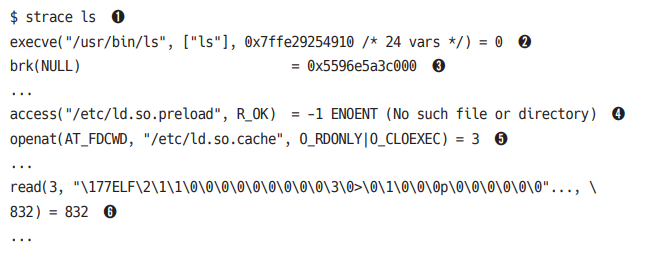
\includegraphics[width=15cm]{resource/strace-example.png}
    \caption{ls 내부 동작}
\end{figure}

\begin{enumerate}
    \item strace에 ls가 사용하는 시스템 콜을 기억하도록 요청한다.
        실제로는 상당히 길기 때문에 생략된 예시이다.
    \item execve 시스템 콜은 /usr/bin/ls를 실행해 셸 프로세스를 교체한다.
    \item brk 시스템 콜은 메모리를 할당하는 오래된 방식이다.
        malloc을 사용하는 것이 더 안전하고 이식성이 좋다.
        malloc은 시스템 콜이 아니며, mallocopt를 사용하여 접근한 메모리 양에 따라
        brk 시스템 콜 혹은 mmap 시스템 콜을 사용해야 하는지 여부를 결정하는 함수이다.
    \item access 시스템 콜은 프로세스가 특정 파일에 접근할 수 있는지 확인한다.
    \item openat 시스템 콜은 O\_RDONLY|O\_CLOEXEC 플래그(마지막 인수)를 사용해
        디렉터리 파일 디스크립터(여기서 첫 번째 인수인 AT\_FDCWD, 현재 디렉터리를 나태냄)와
        관련된 /etc/ld.so.cache 파일을 연다.
    \item read 시스템 콜은 파일 디스크립터(첫 번째 인수, 3)로 부터 832바이트(마지막 인수)를
        버퍼(두 번째 인수)로 읽는다.
\end{enumerate}

\begin{flushleft}
    strace는 사용자 영역과 커널 사이에 이벤트 라이브 스트림을 가로채는 방식으로
    어떤 시스템 콜이 어떤 순서로 어떤 인수를 사용해 호출되었는지 정확하게 파악하기 위해 유용하다.
    strace는 또한 성능 진단에도 유용하다. curl 명령이 어디서 대부분의 시간을 소비하는지 살펴보자.
\end{flushleft}

\begin{figure}
    \centering
    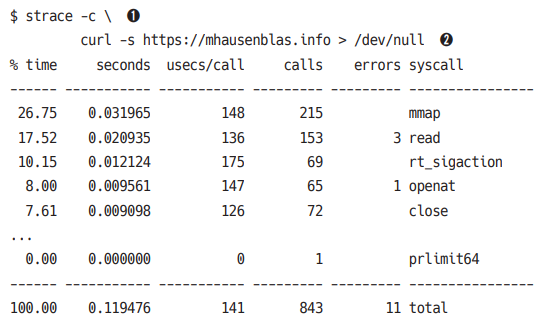
\includegraphics[width=10cm]{resource/strace-example2.png}
    \caption{curl 수행 시간 분석}
\end{figure}

\begin{enumerate}
    \item -c 옵션을 사용하여 사용된 시스템 콜의 개요 통계를 작성한다.
    \item curl의 출력물 모두 버린다.
\end{enumerate}

\begin{flushleft}
    아래의 표는 커널 구성요소와 시스템 전체에 걸쳐 널리 사용되는 시스템 콜 목록이다.
    \href{https://www.man7.org/linux/man-pages/dir_section_2.html}{매뉴얼 페이지}를 참고하여 보다 상세한 시스템 콜 정보를 확인할 수 있다. 
\end{flushleft}

\begin{table}[H]
    \everyrow{\hline}
    \begin{tabu}{|X[1]|X[4]|}
        카테고리 & 시스템 콜 예시 \\
        프로세스 관리 & clone, fork, execve, wait, exit, getpid, 
                            setuid, setns, getrusage, capset, ptrace \\
        메모리 관리 & brk, mmap, munmap, mremap, mlock, mincore \\
        네트워킹 & socket, setsockopt, getsockopt, bind, listen,
                        accept, connect, shutdown, recvfrom, recvmsg,
                        sendto, sethostname, bpf \\ 
        파일시스템 & 기타 \\ 
        시간 & time, clock\_settime, timer\_create, alarm, nanosleep \\ 
        시그널 & kill, pause, signalfd, eventdf \\ 
        전역 & uname, sysinfo, syslog, acct, \_sysctl, iopl, reboot \\
    \end{tabu}
    \caption{시스템 콜 예시}
\end{table}
\newpage

\section{커널 확장}
\begin{flushleft}
    대체로 일상적인 작업에 필요하지 않지만, 커널 고급 주제이다.
    주로 커널을 확장하는 방법에 중점을 둔다.
\end{flushleft}

\begin{flushleft}
    쉬운 내용부터 시작하자.
    현재 사용중인 커널을 다음의 명령을 사용해 간단히 확인할 수 있다.
\end{flushleft}

\begin{figure}[h]
    \centering
    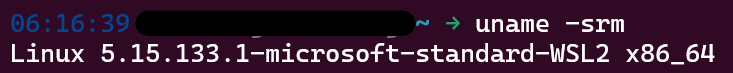
\includegraphics[width=10cm]{resource/uname-example.png}
    \caption[left]{uname 예제}
    \begin{itemize}
        \item 이 uname 출력값을 통해 5.15 커널을 사용하고 있음을 알 수 있다.
    \end{itemize}
\end{figure}

\begin{flushleft}
    이제 커널 버전을 알았으니, 커널 소스 코드에 기능을 추가해서 빌드하지 않고도
    커널 외부로 학장하는 방법에 대한 문제를 해결할 수 있다.
    이렇게 확장하려면 모듈을 사용할 수 있다.
\end{flushleft}

\subsection*{모듈}
\begin{flushleft}
    \textbf{모듈}은 요청 시 커널에 로드할 수 있는 프로그램이다.
    즉, 커널을 다시 컴파일하거나 시스템을 재부팅할 필요가 없다.
    최근 리눅스는 대부분의 하드웨어를 자동으로 감지해 해당 모듈을 자동으로 로드한다.
    하지만, 수동으로 로드하고 싶은 경우도 있다.
    예를 들어 제조사의 모듈 대신 서드파티 모듈을 사용하려는 경우이다.
\end{flushleft}

\begin{flushleft}
    다음 명령을 실행하면 실행 가능한 모듈을 나열할 수 있다.
\end{flushleft}

\begin{figure}[h]
    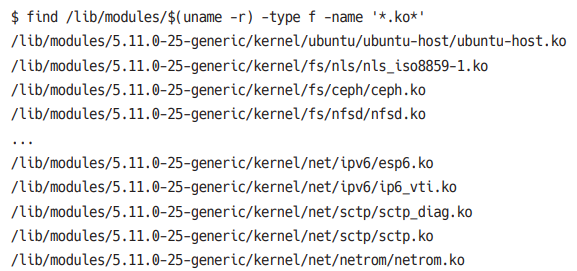
\includegraphics[width=10cm]{resource/module-1.png}
\end{figure}
\newpage

\begin{flushleft}
    그 다음 실제로 로드한 모듈을 확인해보자.
\end{flushleft}

\begin{figure}[h]
    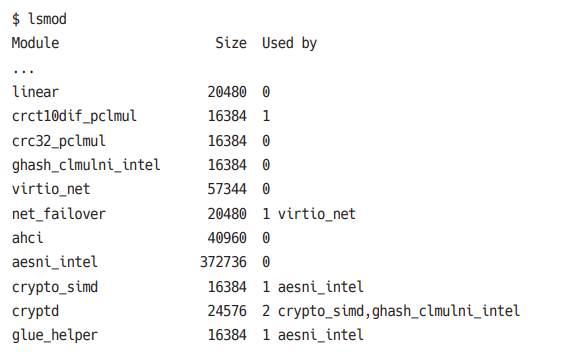
\includegraphics[width=10cm]{resource/module-2.png}
\end{figure}

\begin{flushleft}
    이 정보는 /proc/modules를 통해 볼 수 있다는 것을 주목하라.
    이는 의사 파일시스템 인터페이스를 통해 정보를 노출하는 커널 덕분이다.
    다음은 커널을 확장하는 현대적 대안인 eBPF이다.
\end{flushleft}

\subsection*{커널을 확장하는 현대적인 방법: eBPF}
\begin{flushleft}
    요즘 커널 기능 확장으로 eBPF(아무 의미 없음)가 인기를 끌고 있다.
    원래 BPF(Berkeley Packet Filter)로 불렸다.
\end{flushleft}

\begin{flushleft}
    기술적으로 eBPF(아무 의미 없음)는 리눅스 커널의 기능이며,
    이를 활용하기 위해 커널 3.1.5 이상 버전이 필요하다.
    시스템 콜을 사용해 커널 기능을 안전하고 효율적으로 확장한다.
    eBPF는 맞춤형 RISC 64-bit ISA를 사용한 커널 내 가상 머신으로 구현되었다.
\end{flushleft}

\begin{figure}[h]
    \centering
    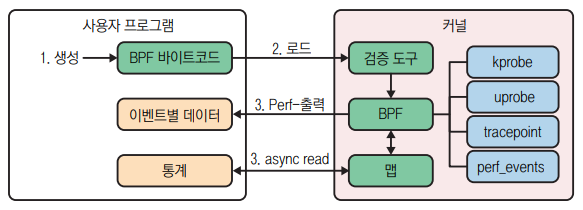
\includegraphics[width=15cm]{resource/2-5.png}
    \caption{리눅스 커널의 eBPF 개요}
\end{figure}
\newpage

\begin{flushleft}
    eBPF는 이미 다양한 곳에서 사용되고 있다.
\end{flushleft}

\begin{itemize}
    \item \textbf{쿠버네티스에서 포드 네트워킹(pod networking)을 활성화하기 위한 CNI 플러그인}\newline
        대표적인 예로, 실리움과 프로젝트 칼리코에서 사용된다.
        또한 서비스 확장성을 위해서도 사용된다.
    \item \textbf{관측가능성용}\newline
        iovisor/bpftrace 같은 리눅스 커널 추적과
        허블(Hubble)을 사용한 클러스터 설정을 위해 사용된다.
    \item \textbf{보안 제어 역할}\newline
        컨테이너 런타임 스캔을 수행할 때 사용할 수 있다.
    \item \textbf{네트워크 로드밸런싱용}\newline
        로드밸런서로도 사용할 수 있다.
\end{itemize}
